\section{Результаты}
\textbf{Примеры работы программы:}
\begin{center}

\includegraphics[width=.49\textwidth]{1}\hfill
\includegraphics[width=.49\textwidth]{1_out}

\includegraphics[width=.49\textwidth]{cat}\hfill
\includegraphics[width=.49\textwidth]{cat_out}

\includegraphics[width=.49\textwidth]{cska}\hfill
\includegraphics[width=.49\textwidth]{cska_out}

\end{center}
В качестве тестовых данных было взято квадратное изображение заданного размера. Пиксели генерировались с помощью генератора псевдослучайных чисел.

Для сравнения я написал программу, использующую только $CPU$, работающую в однопоточном режиме. 
Очевидно, что программа на $GPU$ будет кратно быстрее, поэтому я разделил графики замеров работы.

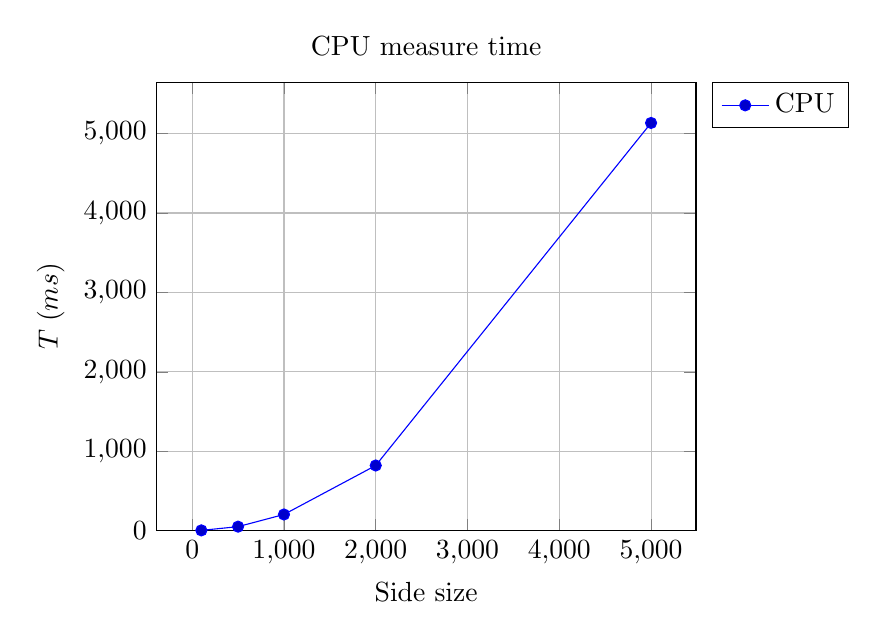
\begin{tikzpicture}% coordinates
	\begin{axis}[
		title = CPU measure time,
		xlabel=Side size,
		ylabel= $T\;(ms)$,
		ymin = 0,
		grid=major,
		legend pos = outer north east
		]
		\legend{CPU}
		\addplot coordinates {(100, 1.902463) (500, 48.8273754) (1000, 202.0314580) (2000, 819.271000) (5000, 5135.031290)};
	\end{axis}
\end{tikzpicture}

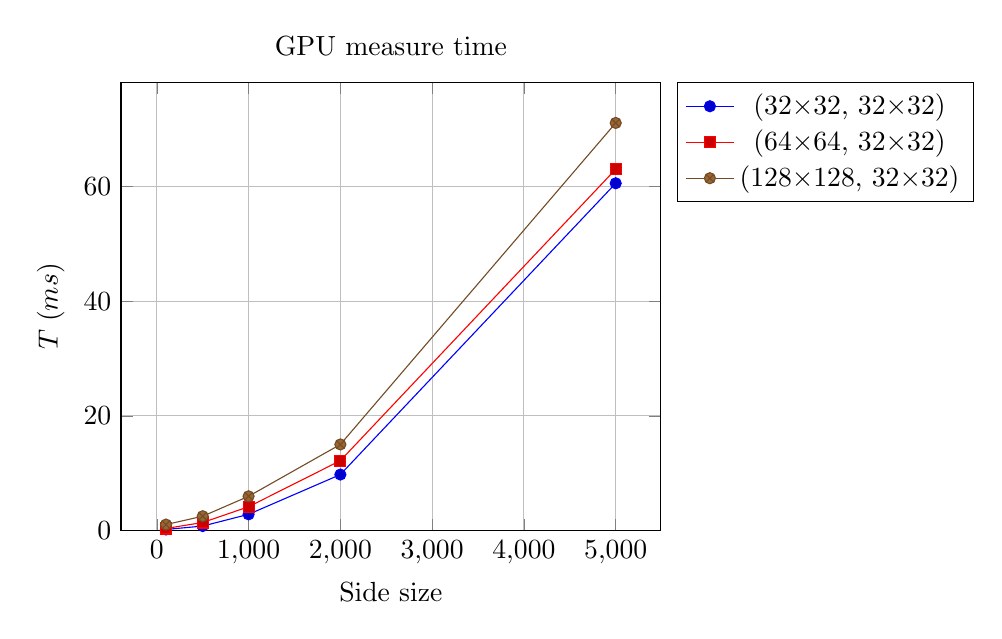
\begin{tikzpicture}% coordinates
	\begin{axis}[
		title = GPU measure time,
		xlabel=Side size,
		ylabel= $T\; (ms)$,
		ymin = 0,
		grid=major,
		legend pos = outer north east
		]
		\legend{(32$\times$32, 32$\times$32), (64$\times$64, 32$\times$32), (128$\times$128, 32$\times$32)}
		\addplot coordinates {(100, 0.183968 ) (500,  0.774368 ) (1000, 2.823550) (2000, 9.764260) (5000, 60.597000)};
		\addplot coordinates {(100, 0.356704) (500,  1.397250 ) (1000, 4.145730) (2000, 12.191700 ) (5000, 63.058200)};
		\addplot coordinates {(100, 1.035650 ) (500,  2.492030 ) (1000, 5.967460 ) (2000, 15.019600) (5000, 71.128200)};
	\end{axis}
\end{tikzpicture}